\section{Giới thiệu ELK-stack}
ELK Stack là từ viết tắt được sử dụng để mô tả bộ dịch vụ bao gồm 3 dự án phổ biến: Elasticsearch, Logstash và Kibana. Thường được gọi là Elasticsearch, ELK Stack mang tới khả năng tổng hợp log từ tất cả các hệ thống và ứng dụng của bạn, phân tích những log này, hiển thị dữ liệu để giám sát ứng dụng và cơ sở hạ tầng, khắc phục sự cố nhanh hơn, phân tích bảo mật, v.v. Không quan trọng webserver sử dụng NGINX, Apache hay MSServer, không quan trọng log đến từ ứng dụng, database, cache server... chúng đều có thể được xử lý bởi ELK!

\begin{figure}[H] % places figure environment here   
    \centering % Centers Graphic
    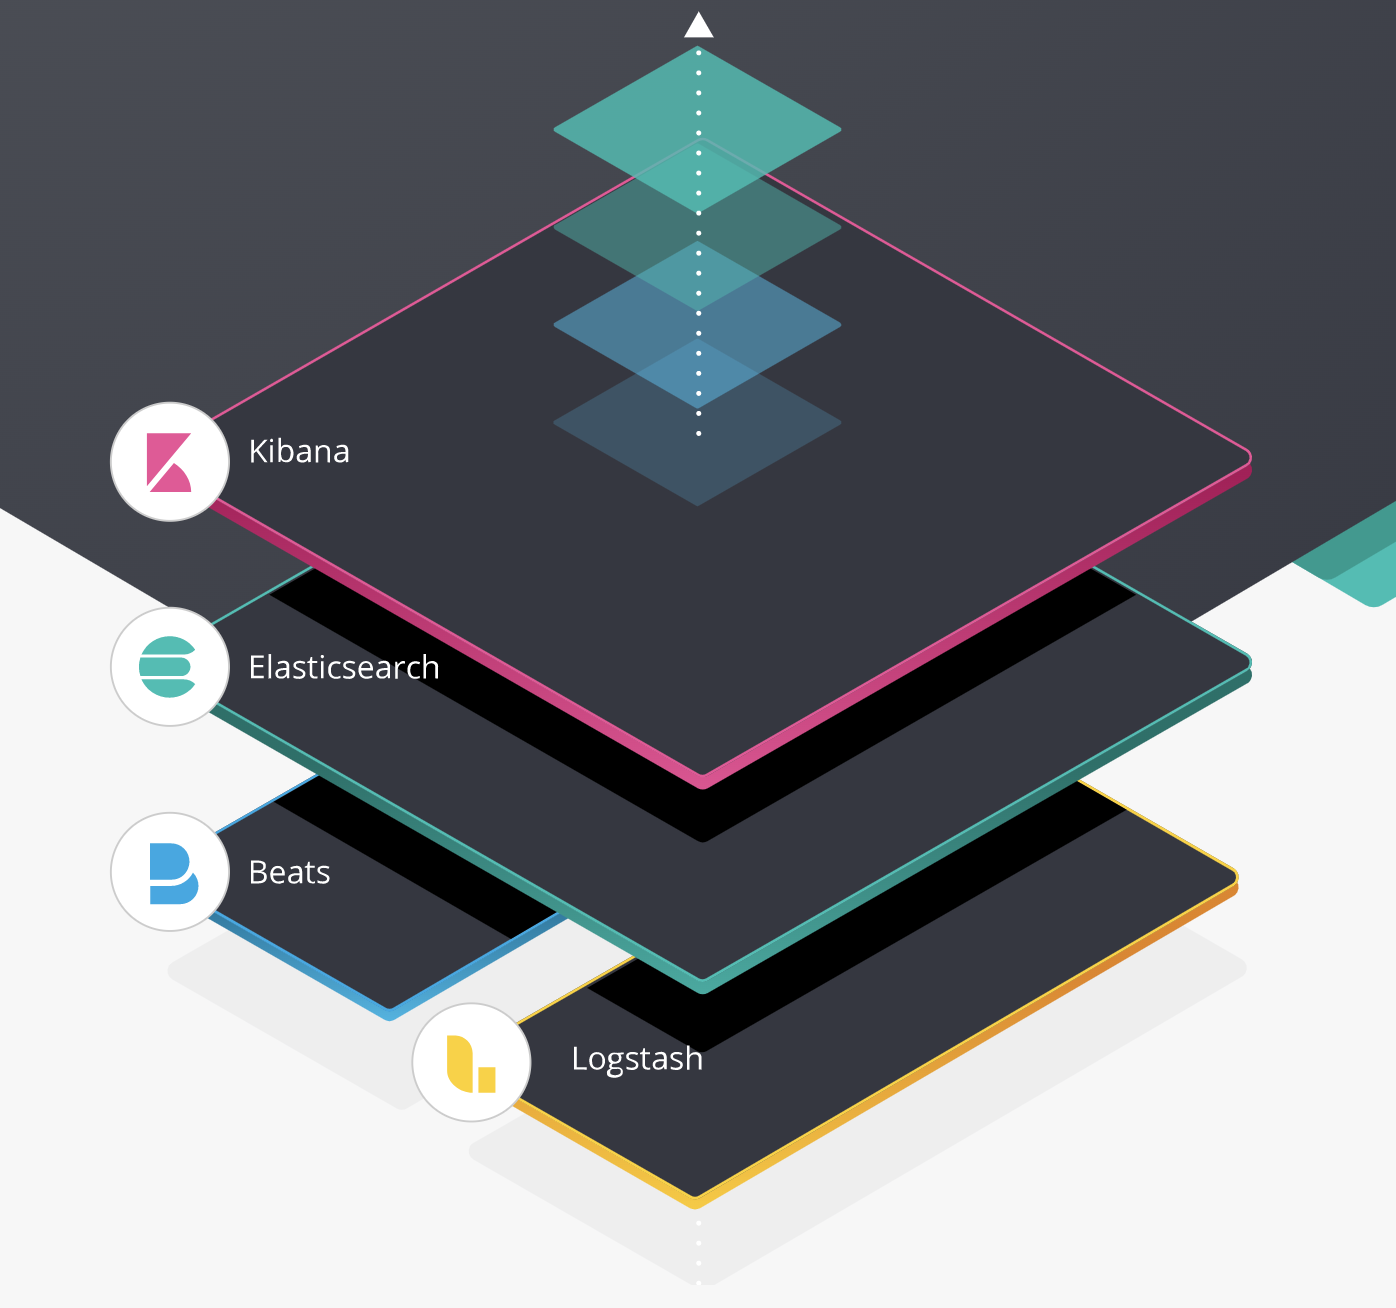
\includegraphics[width=0.8\textwidth]{figures/elk_02.png} 
    \caption{ELK stack} % Creates caption underneath graph
    \label{fig:elk_02}
\end{figure}

\begin{itemize}
    \item \textit{E = Elasticsearch}: Elasticsearch là công cụ tìm kiếm và phân tích phân tán được xây dựng trên Apache Lucene. Khả năng hỗ trợ đa dạng ngôn ngữ, hiệu suất cao và JSON doccument phi cấu trúc khiến Elasticsearch trở thành một lựa chọn lý tưởng cho nhiều trường hợp sử dụng tìm kiếm và phân tích log khác nhau.
    \item \textit{L = Logstash}: Logstash là một công cụ thu nạp dữ liệu nguồn mở cho phép thu thập dữ liệu từ các nguồn khác nhau, chuyển đổi dữ liệu và gửi dữ liệu tới điểm đích. Với các bộ lọc được tạo sẵn và hỗ trợ hơn 200 phần bổ trợ, Logstash cho phép người dùng dễ dàng thu nạp bất kỳ dữ liệu đến từ nguồn hay thuộc loại dữ liệu nào.
    \item \textit{K = Kibana}: Kibana là một công cụ hiển thị trực quan và khám phá dữ liệu dành cho hoạt động đánh giá log và sự kiện. Kibana cung cấp các biểu đồ tương tác dễ sử dụng, các bộ lọc được tạo sẵn cũng như hỗ trợ không gian địa lý. 
\end{itemize}

\begin{figure}[H] % places figure environment here   
    \centering % Centers Graphic
    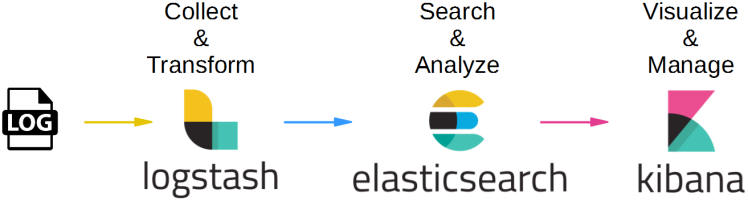
\includegraphics[width=0.6\textwidth]{figures/elk_01.png} 
    \caption{ELK stack với log ứng dụng} % Creates caption underneath graph
    \label{fig:elk_01}
\end{figure}
Nói một cách đơn giản thì Logstash là nơi tiếp nhận dữ liệu từ nhiều nguồn sau đó có thể biến đổi hoặc lọc bớt dữ liệu và ghi vào Elasticsearch. Elasticsearch vừa là nơi lưu trữ vừa là công cụ có khả năng tìm kiếm và phân tích. Kibana là công cụ trực quan hoá dữ liệu từ Elasticsearch, ngoài ra nó cũng cung cấp giao diện đơn giản để thực hiện truy vấn, phân tích với Elasticsearch dễ dàng hơn.

Câu hỏi đặt ra là tại sao ta lại cần một hệ thống \textit{cồng kềnh} như Elasticsearch? Đương nhiên với hệ thống nhỏ, ta chỉ cần ghi log ra file là xong, tuy nhiên với những hệ thống lớn, triển khai trên nhiều servers với nhiều services khác nhau ta không thể nào truy cập vào từng instance của từng service để đọc log, điều tra lỗi. Mặt khác log chứa rất nhiều thông tin của ứng dụng mà đôi khi ta không phải lúc nào cũng muốn ghi xuống cơ sở dữ liệu (thường chậm hơn nhiều so với việc ghi log). Vậy để tổng hợp, phân tích những metrics đó, những công cụ mặc định của hệ điều hành là không đủ. ELK sinh ra để giải quyết tất cả những vấn đề đó bằng việc tập trung toàn bộ log vào Elasticsearch, nơi có thể trực quan hóa, tổng hợp, phân tích, tìm kiếm một cách hết sức thuận tiện. Ngoài ra với hiệu năng truy vấn đáng nể, Elasticsearch còn có thể được sử dụng như một \textit{search engine}. Tuy nhiên trong khuôn khổ bài báo cáo này, tác giả chỉ tập trung đến khả năng thu thập, trực quan hóa và case study về điều tra lỗi thay vì đề cập nhiều đến khả năng truy vấn (vốn là tính năng mạnh mẽ nhất của Elasticsearch). 